\documentclass[fleqn, 11pt]{article}
\usepackage{float}
\usepackage{graphicx}
\usepackage[portuges]{babel}
\usepackage[utf8x]{inputenc}
\usepackage{comment}
\usepackage{fullpage}
\usepackage{xcolor}
\usepackage{amsmath,amsfonts,amssymb,amsthm, bm}

\usepackage{listings}
\usepackage{color}
\definecolor{mygreen}{RGB}{28,172,0}
\definecolor{mylilas}{RGB}{170,55,241}
\renewcommand{\min}{\expandafter\,\operatorname*{min}}

\begin{document}
\noindent
\large\textbf{Lista de Exercícios 1} \hfill \textbf{Luis Vinicius Costa Silva} \\
\normalsize Otimização Clássica \\
Prof. Romes Antonio Borges \\
\hfill Data de Entrega: 29/05/2019

%\section{Questão 1}
%Considere um peso de 500N suspenso por um cabo, como mostra a Figura \ref{figure:fig1}. Uma força $F = 100 N$ é aplicada no peso. Sob o efeito dessa força, o peso move-se da posição original $A$ para uma nova posição de equilíbrio $B$. A posição de equilíbrio é tal que a energia potencial $PE$ é mínima, onde $PE = WY-FX$

%\begin{figure}[!htb]
%\label{figure:fig1}
%   \center{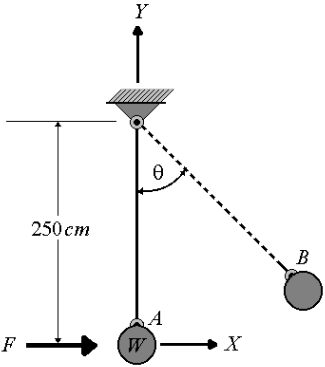
\includegraphics[width=0.33\textwidth]{pendulo.png}}
%   \caption{}
%\end{figure}


%\subsection{Escreva uma expresssão para $PE$ em termos somente do deslocamento $X$.}
%\begin{align*}
%PE = WY-FX \\
%FX + PE = WY \\
%X = \frac{WY - PE}{F} 
%\end{align*}

%\subsection{Escreva uma expressão para $PE$ em termos somente do ângulo $\theta$}
%\begin{align*}
%PE = WY-FX = mgh \\
%h = L(1-\cos{\theta}) \\
%\theta = 2 \pi n - cos^{-1} \bigg( 1-\frac{h}{L} \bigg )
%\end{align*}
%onde $L$ é o comprimento da corda do pêndulo.

%\subsection{Plote um gráfico de $PE$ versus $\theta$, entre $\theta=0^0$ e $\theta = 45^0$.}
\section*{Questão 2}
Considerando a função
\begin{align*}
\begin{split}
f(x_1, x_2) = \pi [3(x_1-x_2)-\sqrt{(3x_1+x_2)(x_1+3x_2)}]
\end{split}
\end{align*}
temos que:


\begin{align*}
\vec{\nabla} f(x_1, ..., x_n) = \biggl( \frac{\partial f}{\partial x_1}, ..., \frac{\partial f}{\partial x_n} \biggr) \end{align*}
Logo, 

\begin{align*}
\vec{\nabla} f(x_1, x_2) = 
\begin{split}
\biggr [\biggr ( \pi \biggr (\frac{-3x_1-5x_2}{\sqrt{3x_{{1}}^2+10x_{1}x_{2}+3x_2^2}} + 3 \biggl ) \biggl ), 
\biggr ( \pi \biggr (\frac{-5x_1-3x_2}{\sqrt{3x_{{1}}^2+10x_{1}x_{2}+3x_2^2}} - 3
\biggl )
\biggl )
 \biggl ]
\end{split}
\end{align*}

Para $p_1 = (0.3, 0.4)$ temos que:
\begin{align*}
\vec{\nabla} f(p_{{1}_{x}}, p_{{1}_{y}}) = (2.90053, -15.4991)
\end{align*}
e a direção de máxima descida $S$: 

\begin{align*}
S = -\vec{\nabla} f(p_{{1}_{x}}, p_{{1}_{y}}) = (-2.90053, 15.4991)
\end{align*}

A matriz Jacobiana computada da seguinte forma:

$$
J(f(x)) = 
  \begin{bmatrix}
  \frac{\partial f_1}{x_1} &  &  & &  &  \frac{\partial f_1}{x_m} \\
   & & ...  & & & \\
   & & ...  & & & \\
   & & ...  & & & \\
   & & ...  & & & \\
 \frac{\partial f_n}{x_1} &   & \phantom{-2}  &  &   &  \frac{\partial f_n}{x_m}
  \end{bmatrix}
$$
Neste caso, temos que a matriz jacobiana de $f$ original é:

$$
\begin{bmatrix}
 \pi \biggr (\frac{-3x_1-5x_2}{\sqrt{3x_{{1}}^2+10x_{1}x_{2}+3x_2^2}} + 3 \biggl )
 & 
 \pi \biggr (\frac{-5x_1-3x_2}{\sqrt{3x_{{1}}^2+10x_{1}x_{2}+3x_2^2}} - 3
\biggl )
\end{bmatrix}
$$

A Hessiana é computada da seguinte forma:

\begin{align*}
\begin{split}
H(f(x)) =
\begin{bmatrix}
\frac{\partial f}{\partial^{2} x} & \frac{\partial f}{\partial x \partial y} \\ 
\frac{\partial f}{\partial y \partial x} & \frac{\partial f}{\partial^{2} y}
\end{bmatrix}
\end{split}
\end{align*}



Logo, a Hessiana desta função é:

\begin{align*}
\begin{split}
H(f(x)) =
\begin{bmatrix}
\frac{16 \pi x_2 ^{2}}{(3x_1 ^{2}+10x_1 x_2 +3x_2 ^{2})^{\frac{3}{2}}} & -\frac{16 \pi x_1  x_2 }{(3 x_1 ^2 + 10 x_1  x_2  + 3 x_2 ^2)^{3/2}} \\
-\frac{16 \pi x_1  x_2 }{(3 x_1 ^2 + 10 x_1  x_2  + 3 x_2 ^2)^{3/2}} & \frac{16 \pi x_1 ^{2}}{(3x_1 ^{2}+10x_1 x_2 +3x_2 ^{2})^{\frac{3}{2}}}
\end{bmatrix}
\end{split}
\end{align*}

As curvas de nível tangenciando a superfície da função podem ser observadas abaixo, assim como o o vetor de descida máxima da função (i.e: $S = -\nabla f(x_1, x_2)$)

\begin{figure}[H]
\label{figure:fig1}
   \center{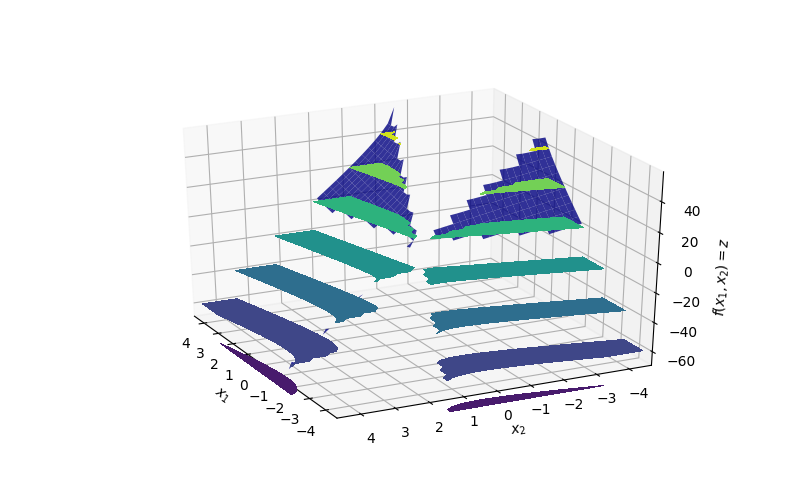
\includegraphics[width=\textwidth]{2_contorno.png}}
   \caption{Curvas de nível e superfície da função, assim como o vetor de descida máxima}
\end{figure}
\begin{figure}[H]
\label{figure:fig1}
   \center{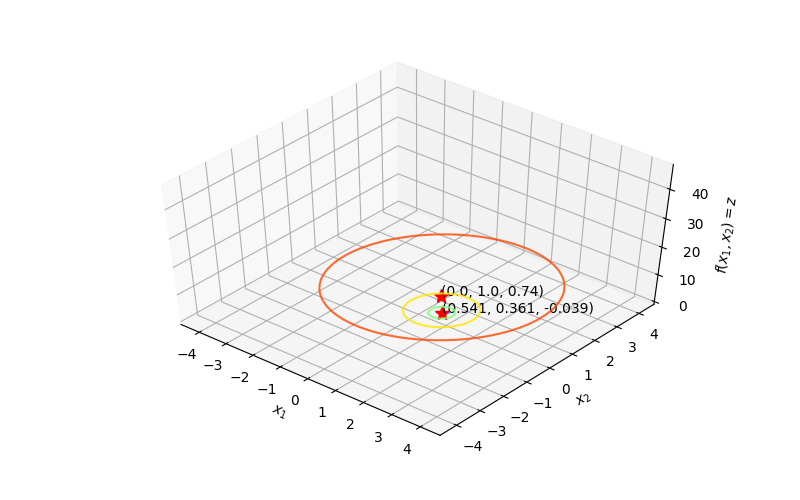
\includegraphics[width=\textwidth]{3_2_contorno.png}}
   \caption{Curvas de nível, em destaque temos o ponto de máximo global da mesma}
\end{figure}


\newpage
\section*{Questão 3}
Considerando a função

\begin{align*}
\begin{split}
f(x_1,x_2) = -\pi  (0.072) x_{1} x_{2} + (x_{1}-0.5)^{2} + (x_{2}-0.3)^2
\end{split}
\end{align*}
Temos que:
\begin{align*}
\begin{split}
\frac{\partial f}{\partial 	x_1} = 2x_{1} - 0.226195 x_{2} - 1
\end{split}
\end{align*}

\begin{align*}
\begin{split}
\frac{\partial f}{\partial 	x_2} = 2x_{1} - 0.226195 x_{2} - 1
\end{split}
\end{align*}

\begin{align*}
\begin{split}
\frac{\partial f}{\partial x^2} = \frac{\partial f}{\partial y^2} = 2
\end{split}
\end{align*}

\begin{align*}
\begin{split}
\frac{\partial f}{\partial 	x_1 x_2} =\frac{\partial f}{\partial 	x_2 x_1} = -0.226195
\end{split}
\end{align*}

Logo, a Hessiana é igual a:

\begin{align*}
H(f(x)) =
\begin{bmatrix}
2 & -0.226195 \\ 
-0.226195 & 2
\end{bmatrix}
\end{align*}

Visto que $\det([2]) = 2$ e $\det(H(f(x))) = 3.9488...$, temos que esta matriz Hessiana é positiva definida.
\begin{figure}[H]
\label{figure:fig1}
   \center{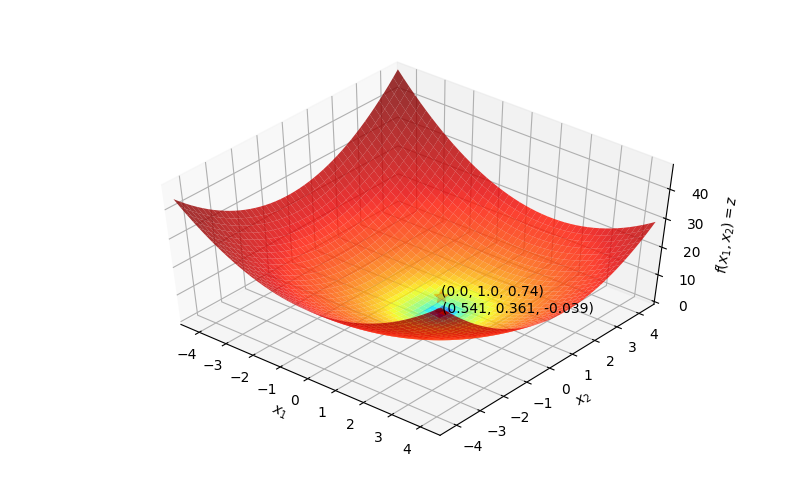
\includegraphics[width=\textwidth]{3_2_superficie.png}}
   \caption{Superfície da função, em destaque temos o ponto de máximo e mínimo local da mesma}
\end{figure}

\newpage
\section*{Questão 5}
Dado o problema:
\begin{align*}
\begin{split}
\min x_1 + \frac{1}{x_1}+x_2+\frac{1}{x_2}
\end{split}
\end{align*}

\begin{align*}
\begin{split}
\text{Temos que o gradiente de uma função é dado por:}
\end{split}
\end{align*}

\begin{align*}
\begin{split}
\vec{\nabla} f (x_1, ..., x_n) = \biggl( \frac{\partial f}{\partial x_1}, ..., \frac{\partial f}{\partial x_n} \biggr)
\end{split}
\end{align*}

\begin{align*}
\begin{split}
\text{logo...}
\end{split}
\end{align*}

\begin{align*}
\begin{split}
\vec{\nabla} f(x_1,x_2) = [1 - x_{1}^{-2}, 1 - x_{2}^{-2}]
\end{split}
\end{align*}
A Hessiana é computada da seguinte forma:

\begin{align*}
\begin{split}
H(f(x)) =
\begin{bmatrix}
\frac{\partial f}{\partial^{2} x} & \frac{\partial f}{\partial x \partial y} \\ 
\frac{\partial f}{\partial y \partial x} & \frac{\partial f}{\partial^{2} y}
\end{bmatrix}
\end{split}
\end{align*}
Logo, a Hessiana desta função é:

\begin{align*}
H(f(x)) =
\begin{bmatrix}
2{x_{1}}^{-3} & 0 \\ 
0 & 2{x_{2}}^{-3}
\end{bmatrix}
\end{align*}
Os valores que tornam $\vec{\nabla} f(x) = 0$ são obtidos através da solução do sistema abaixo:

\begin{align*}
\left(\{\begin{matrix}
1-x_1^{-2} = & 0 \\ 
1-x_2^{-2} = & 0 
\end{matrix}\right.
\end{align*}
Temos que $x_1 = x_2 = \pm 1 \leftrightarrow  x_1 = x_2$ senão $x_1 = -x_2$, tal que $x_1 = \pm 1$.

Observa-se que os pontos $p_1 = (-1, -1)$ e $p_2 = (1, 1)$ são respectivamente o máximo e mínimo local, visto que $H(f(p_{1_{x}}, p_{1_{y}})) < 0$ assim como $H(f(p_{2_{x}}, p_{2_{y}})) > 0$
\end{document}